\documentclass[
aspectratio=3218, 
10pt, hyperref={pdfpagelabels=false}]{beamer}

\usepackage{CJKutf8}
\usepackage[english]{babel}
\usepackage{xcolor}
\usepackage{lmodern}
\usepackage{amssymb}
%\usefonttheme{serif}
\usepackage[makeroom]{cancel} %for crossing symbols
\usepackage{leftindex} %For leftindex, making it possible to have nicely aligned left subscripts
%\usepackage{calligra}
%\DeclareMathAlphabet{\mathcalligra}{T1}{calligra}{m}{n} %For small \mathcal letters
\makeatletter
\DeclareFontEncoding{LS1}{}{}
\DeclareFontSubstitution{LS1}{stix}{m}{n}
\DeclareMathAlphabet{\mathKel}{LS1}{stixscr}{m}{n}
\DeclareMathAlphabet{\mathcal}{LS1}{stixscr}{m}{n}
\usepackage{amsthm}
\usepackage{amsmath}
%\usepackage{mathabx}
\usepackage{stmaryrd}
\usepackage{amsbsy}
\usepackage{dsfont}
\usepackage{mathtools} %für mathclap und coloneqq
%\usepackage{amsbsy}
\usepackage{mleftright} %Distanz zu \left \right weg
\usepackage{tikz-cd}

\usepackage{tabularx} %Automatic line break of tables using X instead c l r
%\usepackage{longtable} %table auf mehreren Seiten
%\usepackage{ltxtable} %Combination of both above
\usepackage{xcolor, colortbl}

%Für die ganzen Diagramme
\usepackage{pgfplots}

\usepackage{appendixnumberbeamer}

\usepackage{booktabs}
\usepackage[scale=2]{ccicons}

\usepgfplotslibrary{dateplot}
\usetikzlibrary{fit,
                shapes.arrows}

\usepackage{xspace}

\usepackage{graphicx} %Für raisebox, vertical displacement of figures
\usetikzlibrary{decorations.markings, decorations.text,calc,arrows.meta}

\definecolor{Gray}{gray}{0.85}
%\usepackage[style=authortitle-icomp]{biblatex}
%\usepackage[babel,german=guillemets]{csquotes}

%\setcounter{tocdepth}{1}
%\setcounter{tocdepth}{5}
%\setcounter{secnumdepth}{4}
%\setcounter{secnumdepth}{5}
\usepackage[backend=biber, style=numeric]{biblatex}
\addbibresource{Literatur.bib}
\newcommand\fibtimes[2]{\mathbin{_{#1}\times_{#2}}}
%\newcommand{\footlineextra}[1]{
    %\begin{tikzpicture}[remember picture,overlay]
        %\node[yshift=2ex,anchor=south west] at (current page.south west) {\usebeamerfont{author in head/foot}\hspace{2ex}#1};
    %\end{tikzpicture}
%}

%\newcommand\insertreferences{}
%\setbeamertemplate{footline}{%
  %\leavevmode%
  %\hbox{%
  %\begin{beamercolorbox}[wd=.09\paperwidth, ht=5ex,dp=1ex,center, sep=1.4ex]{author in head/foot}%
    %\usebeamerfont{author in head/foot}
		%%\vfill
		%%Sources
		%%\vfill
		%Sources
  %\end{beamercolorbox}%
  %\begin{beamercolorbox}[wd=.91\paperwidth,ht=5ex,dp=1ex,center]{title in head/foot}%
    %\usebeamerfont{title in head/foot}
    %\insertreferences
%
  %\end{beamercolorbox}
%}
%}


%%% Transition slides
%\AtBeginSection[]{
  %\begin{frame}
  %%\vfill
	%\thispagestyle{empty}
  %\centering
  %\begin{beamercolorbox}[sep=8pt,center,shadow=true,rounded=true]{title}
    %\usebeamerfont{title}\insertsection\par%
  %\end{beamercolorbox}
  %%\vfill
  %\end{frame}
%}

\title{Curved Yang-Mills-Higgs theories}   
\subtitle{}   
\author{Simon-Raphael Fischer, \textit{based on joint works with Camille Laurent-Gengoux, and with Mehran Jalali Farahani, Hyungrok Kim (\begin{CJK*}{UTF8}{bkai}金炯錄\end{CJK*}), Christian Sämann}} 
\institute{
\begin{figure}
	\centering
		\includegraphics[width=.50\textwidth]{Logo_Uni_Göttingen_2022.png}
	\label{fig:NCTS}
\end{figure}
\begin{center}
%Mathematical Institute
\end{center}
}
\date{} 
%\date{Le lundi 31 mai 2021} 

% zusaetzlich ist das usepackage{beamerthemeshadow} eingebunden 
%\usepackage{beamerthemeIlmenau}
%\usepackage{beamerthemeshadow}
%\usepackage{beamerthemeDarmstadt}
%\usetheme{Arguelles}
\usetheme{metropolis}
%\usepackage[orientation=landscape,size=custom,width=16,height=9,scale=0.5,debug]{beamerposter}

%  \beamersetuncovermixins{\opaqueness<1>{25}}{\opaqueness<2->{15}}
%  sorgt dafuer das die Elemente die erst noch (zukuenftig) kommen 
%  nur schwach angedeutet erscheinen 
\beamersetuncovermixins{\opaqueness<1>{25}}{\opaqueness<2->{15}}
% klappt auch bei Tabellen, wenn teTeX verwendent wird\ldots

\beamertemplatenavigationsymbolsempty %Damit sind die kleinen Navigationssymbole unten weg

%\usesectionheadtemplate{}{}
%\usesubsectionheadtemplate{}{}

\def\be{\begin{equation}}
\def\ee{\end{equation}}
\def\bs{\begin{subequations}}
\def\es{\end{subequations}}
\def\ba#1\ea{\begin{align}#1\end{align}}
\def\bes{\begin{equation*}}
\def\ees{\end{equation*}}
\def\bas#1\eas{\begin{align*}#1\end{align*}}

\AtBeginEnvironment{remark}{%
  \setbeamercolor{block title}{use=example text,fg=black,bg=yellow!75!black}
  \setbeamercolor{block body}{parent=normal text,use=block title example,bg=yellow!10}
}
\AtBeginEnvironment{motivation}{%
  \setbeamercolor{block title}{use=example text,fg=black,bg=yellow!75!black}
  \setbeamercolor{block body}{parent=normal text,use=block title example,bg=yellow!10}
}

\renewcommand{\qedsymbol}{}
\theoremstyle{plain}
\newtheorem{conjecture}[theorem]{Conjecture}
\newtheorem{proposition}[theorem]{Proposition}
%\newtheorem{definition}[theorem]{Definition}
\theoremstyle{remark}
\newtheorem*{remark}{Remarks}
\newtheorem*{gedankenexperiment}{Gedankenexperiment}
\newtheorem*{idea}{Idea}
\newtheorem*{motivation}{Motivation}
\newtheorem*{summary}{Summary}
\newtheorem*{situation}{Situation}
\newtheorem*{lab}{Situation: Lie algebra bundles}
\newtheorem*{question}{Question}
\newtheorem*{fieldredefinition}{Field Redefinition}
\newtheorem*{construction}{Construction}
\newtheorem*{aim}{Aim}
\newtheorem*{BackToTheRoots}{Back to the roots}

\AtBeginEnvironment{BackToTheRoots}{%
  \setbeamercolor{block title}{use=example text,fg=black,bg=pink!75!black}
  \setbeamercolor{block body}{parent=normal text,use=block title example,bg=pink!10}
}
\AtBeginEnvironment{gedankenexperiment}{%
  \setbeamercolor{block title}{use=example text,fg=black,bg=pink!75!black}
  \setbeamercolor{block body}{parent=normal text,use=block title example,bg=pink!10}
}
\AtBeginEnvironment{idea}{%
  \setbeamercolor{block title}{use=example text,fg=black,bg=pink!75!black}
  \setbeamercolor{block body}{parent=normal text,use=block title example,bg=pink!10}
}

%\theoremstyle{definition}
%\newtheorem{definition}[theorem]{Definition}
%\newtheorem*{SecondIn}{Second Inequality}

%mathrm mit mathup ersetzen, damit die font passt
\renewcommand\familydefault{\sfdefault} %comment to see the difference
\DeclareMathAlphabet      {\mathup}{OT1}{\familydefault}{m}{n}


\begin{document}


\begin{frame}
\thispagestyle{empty}
\titlepage
\end{frame} 


{
\setbeamertemplate{footline}{}
\begin{frame}
%\frametitle{Table of contents}
%\tableofcontents
\thispagestyle{empty}
\begin{figure}[htbp]
	\centering
		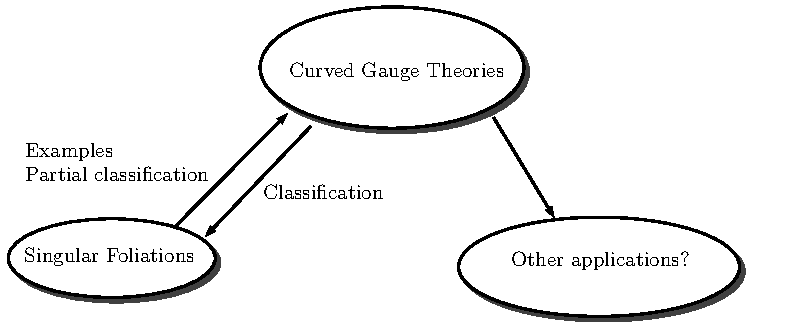
\includegraphics[width=1\textwidth]{Research circles I.pdf}
\end{figure}
\end{frame} 
}

\section{Curved Yang-Mills-Higgs theory}

\subsection{Motivation}



\begin{frame}{Motivation: Covariantisation of Yang-Mills(-Higgs) theory}
\begin{tikzpicture}
\coordinate (a) at (0, 0);
\coordinate (b) at (15, 0);
\path[->, line width=1mm] (a) edge node[above] {Covariantization} (b);
\end{tikzpicture}
{\renewcommand{\arraystretch}{2}
\begin{table}[h!]
		\begin{tabularx}{\textwidth}{c c c}
			\rowcolor{gray}
			Classical theory & Covariantised flat theory & Curved Theory \\
			Vector space $V$ & Trivial vector bundle $M \times V$ & Vector bundle $V \to M$ \\
			\rowcolor{Gray}
			$\frac{\partial}{\partial x^i}$ & Canonical flat connection $\nabla^0$ & Vector bundle connection $\nabla$ \\ 
			\multicolumn{1}{X}{Coordinate changes may lead to extra terms} & 
			\multicolumn{2}{c}{Coordinate expressions form-invariant under coordinate changes}
		\end{tabularx}
\end{table}}

\end{frame}

\setbeamertemplate{frame footer}{S.-R.\ Fischer. \textit{Integrating curved Yang–Mills gauge theories}, arXiv: 2210.02924, 2022. \newline 
S.-R.\ Fischer. \textit{Geometry of curved Yang–Mills–Higgs gauge theories}, Ph.D.\ thesis, Institut Camille Jordan [Villeurbanne], France, U. Geneva, Switzerland, 2021; doi: 10.13097/archive-ouverte/unige:152555}

\begin{frame}{Curved Yang-Mills gauge theory (curved YM theory)}
\begin{tikzpicture}
\coordinate (a) at (0, 0);
\coordinate (b) at (15, 0);
\path[->, line width=1mm] (a) edge node[above] {Covariantization} (b);
\end{tikzpicture}
{\renewcommand{\arraystretch}{2}
\begin{table}[h!]
		\begin{tabularx}{\textwidth}{c c c}
			\rowcolor{gray}
			YM theory & Covariantised YM theory & Curved YM theory \\
			Lie group $G$ & Trivial Lie group bundle $M \times G$ & Lie group bundle $G \to M$ \\
			\rowcolor{Gray}
			Maurer Cartan form & Fibre-wise Maurer-Cartan & Multiplicative YM connection \\ 
			\multicolumn{1}{X}{Field redefinitions lead to extra terms in gauge transformations and field strength} & 
			\multicolumn{2}{c}{Coordinate expressions form-invariant under coordinate changes}
		\end{tabularx}
\end{table}}

\end{frame}

\setbeamertemplate{frame footer}{S.-R.\ Fischer, M.\ Jalali Farahani, H.\ Kim, and C.\ Saemann. \textit{Adjusted connections I: Differential cocycles for principal groupoid bundles with connection}, arXiv: 2406.16755, 202. \newline 
S.-R.\ Fischer. \textit{Geometry of curved Yang–Mills–Higgs gauge theories}, Ph.D.\ thesis, Institut Camille Jordan [Villeurbanne], France, U. Geneva, Switzerland, 2021; doi: 10.13097/archive-ouverte/unige:152555}

\begin{frame}{Curved Yang-Mills-Higgs theory (curved YMH theory)}
\begin{tikzpicture}
\coordinate (a) at (0, 0);
\coordinate (b) at (15, 0);
\path[->, line width=1mm] (a) edge node[above] {Covariantization} (b);
\end{tikzpicture}
{\renewcommand{\arraystretch}{2}
\begin{table}[h!]
		\begin{tabularx}{\textwidth}{c c c}
			\rowcolor{gray}
			YMH theory & Covariantised YMH theory & Curved YMH theory \\
			Lie group $G$ with right-action on $N$ & Action groupoid $N \times G$ & Lie groupoid $G \rightrightarrows N$ \\
			\rowcolor{Gray}
			Maurer Cartan form & Fibre-wise Maurer-Cartan & Covariant adjustments \\ 
			\multicolumn{1}{X}{Field redefinitions lead to extra terms in gauge transformations and field strength} & 
			\multicolumn{2}{c}{Coordinate expressions form-invariant under coordinate changes}
		\end{tabularx}
\end{table}}

\end{frame}

\begin{frame}
\begin{table}[h!]
		\begin{tabularx}{\textwidth}{X X}
			\rowcolor{gray}
			Classical theory & Covariantised flat theory \\
			Lie algebra $\mathfrak{g}$ as $L \times \mathfrak{g}$ & Lie algebroid $E \to N$ \\
			\rowcolor{Gray}
			$\mathfrak{g}$-action $\gamma$ & Anchor $\rho$ of $E$ \\ 
			\rowcolor{Gray}
			& \& $E$-connections \\
			Canonical flat connection $\nabla^0$ on $L \times \mathfrak{g}$ & General connection $\nabla$ on $E$
		\end{tabularx}
\end{table}
\end{frame}




{
\setbeamertemplate{frame footer}{Ana Cannas Da Silva and Alan Weinstein. \textit{Geometric models for noncommutative algebras}, volume 10. American Mathematical Soc., 1999.}

\begin{frame}
\begin{center}
	\begin{tikzcd}[ampersand replacement=\&]
\mathcal{G} \arrow[d, shift left, "s"]\arrow["t", swap, shift right]{d} \\
	M
	\end{tikzcd}
\end{center}

\begin{definition}
$\mathcal{G}$ a \textbf{Lie groupoid} if there are surjective submersions $s, t \colon \mathcal{G} \to M$,  \textit{source} and \textit{target}, respectively, and a smooth \textit{multiplication map} $\mathcal{G} \fibtimes{s}{t} \mathcal{G} \to \mathcal{G}$ such that 
\bes
s(g'g) = s(g), \qquad t(g'g) = t(g')
\ees
for all $(g', g) \in \mathcal{G} \fibtimes{s}{t} \mathcal{G}$ (i.e.\ $s(g') = t(g)$), satisfying the typical expected properties, that is,
\bas
\text{Associativity:} && (g'' g') g &= g'' (g'g),
\\
\text{Units:} && g e_{s(g)} = g, \quad&\quad e_{t(g)} g = g,
\\
\text{Inverse:} && g^{-1} g = e_{s(g)}, \quad&\quad g g^{-1} = e_{t(g)}
\eas
for all $(g'', g', g) \in \mathcal{G} \fibtimes{s}{t} \mathcal{G} \fibtimes{s}{t} \mathcal{G}$, where one requires the existence of the \textit{unit} $e$ as a global section of both, $s$ and $t$, and the \textit{inverse} $g^{-1} \in \mathcal{G}$ of $g$.
\end{definition}
\end{frame}

\begin{frame}
\begin{center}
	\begin{tikzcd}[ampersand replacement=\&]
m'' \& \arrow[l, swap, "g'", bend right] m' \& \arrow[l, swap, "g", bend right] \arrow[ll, swap, "g'g", bend right=70] m
	\end{tikzcd}
\end{center}
\pause
\begin{example}
Lie groups $G$
\begin{center}
	\begin{tikzcd}[ampersand replacement=\&]
G \arrow[d, shift left, "s"]\arrow["t", swap, shift right]{d} \\
	\{*\}
	\end{tikzcd}
\end{center}
\end{example}
\end{frame}

\begin{frame}
\begin{center}
	\begin{tikzcd}[ampersand replacement=\&]
m'' \& \arrow[l, swap, "g'", bend right] m' \& \arrow[l, swap, "g", bend right] \arrow[ll, swap, "g'g", bend right=70] m
	\end{tikzcd}
\end{center}

\begin{example}
Lie group bundles (LGBs) $\pi_G \colon G \to M$
\begin{center}
	\begin{tikzcd}[ampersand replacement=\&]
G \arrow[d, shift left, "\pi_G"]\arrow["\pi_G", swap, shift right]{d} \\
	M
	\end{tikzcd}
\end{center}
\end{example}
\end{frame}

\begin{frame}{Motivation (sort of historical)}
\textbf{We will mainly focus on Yang-Mills theories:}

\begin{table}[h!]
		\begin{tabularx}{\textwidth}{X| c c} 
			\rowcolor{gray}
			& Classical & Curved \\ \hline
			Infinitesimal & Lie algebra $\mathfrak{g}$ & LAB\footnote{LAB = Lie algebra bundle} $\mathcal{g}$ \\
			\rowcolor{Gray}
			Integrated & Lie group $G$ & \textcolor[rgb]{1,0.41,0.13}{LGB\footnote{LGB = Lie group bundle} $\mathcal{G}$} \\
		\end{tabularx}
\end{table}

\vspace{-0.5cm}

\begin{center}
	\begin{tikzcd}[ampersand replacement=\&]
	G \arrow{r} \& \mathcal{G} \arrow{d} \\
	\& L
	\end{tikzcd}
\end{center}

\vspace{-0.5cm}

\pause

\begin{remark}[Why \textbf{curved}?]
For gauge invariance and closure of gauge transformations:

\begin{itemize}
	\item Generalize Maurer-Cartan form $\rightarrow$ \textbf{Multiplicative Yang-Mills connection}.
	\item Generalize Field Strength.
\end{itemize}
\end{remark}

\end{frame}
}

%{
%
%\begin{frame}{Motivation 2 by S.-R.\ F.}
%Consider a semisimple Lie group $G$ and a principal $G$-bundle $P \to L$:
%%$\mathbb{H}$ the horizontal distribution on $\mathcal{P} \tilde{\times} \mathcal{T}$:
%\begin{center}
	%\begin{tikzcd}[ampersand replacement=\&]
	%(P \times \mathfrak{g})/G
	%\arrow[hook]{r}
	%\&
	%\mathup{T}P/G
	%\arrow[two heads]{r}
	%\&
	%\mathrm{T}L \arrow[bend right, swap]{l}{A}
	%\end{tikzcd}
%\end{center}
 %
	%%where $\mathup{Ad}(P)$ and $\mathup{At}(P)$ the adjoint and Atiyah bundle of a principal $G$-bundle $P$, respectively. 
	%\pause
	%
	%\begin{gedankenexperiment}
	%\begin{enumerate}
		%\item Adjoint connection $\leftrightarrow$ Ehresmann connection on $P$. 
		%\item As parallel transport:
		%\begin{equation*}
		%\mathup{PT}_\gamma^{\mathup{Ad}(P)}([p, v])
		%=
		%\mleft[ \mathup{PT}_\gamma^P(p), v \mright]
		%\end{equation*}
		%for all $[p, v] \in (P \times \mathfrak{g})/G$.
	%\end{enumerate}
	%\end{gedankenexperiment}
%\end{frame}
%
%\begin{frame}{Motivation 2 by S.-R.\ F.}
%Consider a semisimple Lie group $G$ and a principal $G$-bundle $P \to L$:
%%$\mathbb{H}$ the horizontal distribution on $\mathcal{P} \tilde{\times} \mathcal{T}$:
%\begin{center}
	%\begin{tikzcd}[ampersand replacement=\&]
	%\mleft(P \times_L \underline{\mathfrak{g}}\mright)/G
	%\arrow[hook]{r}
	%\&
	%\mathup{T}P/G
	%\arrow[two heads]{r}
	%\&
	%\mathrm{T}L \arrow[bend right, swap]{l}{A}
	%\end{tikzcd}
%\end{center}
 %
	%%where $\mathup{Ad}(P)$ and $\mathup{At}(P)$ the adjoint and Atiyah bundle of a principal $G$-bundle $P$, respectively. 
	%
	%\begin{gedankenexperiment}
	%\begin{enumerate}
		%\item Adjoint connection $\leftrightarrow$ Ehresmann connection on $P$. 
		%\item As parallel transport:
		%\begin{equation*}
		%\mathup{PT}_\gamma^{\mathup{Ad}(P)}([p, v])
		%=
		%\mleft[ \mathup{PT}_\gamma^P(p), \mathup{PT}_\gamma^0(v) \mright],
		%\end{equation*}
		%Lie algebra $\mathfrak{g}$ as trivial bundle w/ canonical flat connection
	%\end{enumerate}
	%\end{gedankenexperiment}
%\end{frame}
%
%\begin{frame}{Motivation 2 by S.-R.\ F.}
%Consider a semisimple Lie group $G$ and a principal $G$-bundle $P \to L$:
%%$\mathbb{H}$ the horizontal distribution on $\mathcal{P} \tilde{\times} \mathcal{T}$:
%\begin{center}
	%\begin{tikzcd}[ampersand replacement=\&]
	%\mleft(P \times_L \underline{\mathfrak{g}}\mright)/G
	%\arrow[hook]{r}
	%\&
	%\mathup{T}P/G
	%\arrow[two heads]{r}
	%\&
	%\mathrm{T}L \arrow[bend right, swap]{l}{A}
	%\end{tikzcd}
%\end{center}
 %
	%%where $\mathup{Ad}(P)$ and $\mathup{At}(P)$ the adjoint and Atiyah bundle of a principal $G$-bundle $P$, respectively. 
	%
	%\begin{gedankenexperiment}
	%\begin{enumerate}
		%\item Adjoint connection $\leftrightarrow$ Ehresmann connection on $P$. 
		%\item As parallel transport:
		%\begin{equation*}
		%\mathup{PT}_\gamma^{\mathup{Ad}(P)}([p, v])
		%=
		%\mleft[ \mathup{PT}_\gamma^P(p){\color[rgb]{0.24,0.7,0.44} \cdot \kappa_\gamma}, {\color[rgb]{0.24,0.7,0.44} \kappa_\gamma^{-1} \cdot} \mathup{PT}_\gamma^0(v) \mright],
		%\end{equation*}
		%Lie algebra $\mathfrak{g}$ as trivial bundle w/ canonical flat connection, $\kappa_\gamma$ values in $G$ \& "suitable"
	%\end{enumerate}
	%\end{gedankenexperiment}
%\end{frame}
%
%
%\begin{frame}{Conclusion}
%\begin{block}{Theorem (Field Redefinitions, [S.-R.\ F.])}
%%\begin{itemize}[<+->]
%\vspace{.5pt}
%This leads to an equivalence relation of gauge theories, preserving dynamics and kinematics.
%
%But: In the {\color[rgb]{0.24,0.7,0.44} curved} sense! Curvature terms appear.
%\end{block}
%\pause
%\metroset{block=fill}
%\begin{exampleblock}{Motivation ([S.-R.\ F.])}
%\begin{enumerate}
	%\item How to formulate gauge theory such that it is invariant under field redefinitions?
	%\item Are there curved theories which are \textbf{not} equivalent to classical ones?
%\end{enumerate}
%\end{exampleblock}
%
%
%\end{frame}

%}

%\subsection{Setup}

%\renewcommand\insertreferences{{\tiny  K. Mackenzie. General Theory of Lie Groupoids and Algebroids. \newline \textit{London Mathematical Society Lecture Note Series}, 213, 2005.}}
%
%\begin{frame}
%\begin{definition}[LGB actions, simplified]
%\begin{center}
	%\begin{tikzcd}[ampersand replacement=\&, column sep = small, row sep = small]
	%\& \arrow[bend right]{ld} \mathcal{G} \arrow{d} \\
	%\mathcal{P} \arrow{r}{\pi} \& L
	%\end{tikzcd}
%\end{center}
%$\mathcal{P} \stackrel{\pi}{\to} L$ a fibre bundle. A \textbf{right-action of $\mathcal{G}$ on $\mathcal{P}$} is a smooth map 
%%\bas
%$\mathcal{P} * \mathcal{G} \coloneqq \pi^*\mathcal{G} = \mathcal{P} \times_L \mathcal{G} \to \mathcal{P}$,
%$(p, g) \mapsto p \cdot g$,
%%\eas
%satisfying the following properties:
%\ba\label{InvarianceOffUnderGAction}
%\pi(p \cdot g) &= \pi(p),\\
%(p \cdot g) \cdot h &= p \cdot (gh),\\
%p \cdot e_{\pi(p)} &= p
%\ea
%for all $p \in \mathcal{P}$ and $g, h \in \mathcal{G}_{\pi(p)}$, where $e_{\pi(p)}$ is the neutral element of $\mathcal{G}_{\pi(p)}$.
%\end{definition}
%\end{frame}

%\renewcommand\insertreferences{{\tiny Ieke Moerdijk, Janez Mrcun. Introduction to Foliations and Lie Groupoids. \newline \textit{Cambridge Studies in Advanced Mathematics 91, Cambridge University Press, Cambridge}, 2003}}
%
%\begin{frame}
%\begin{definition}[Principal bundle]
%Still a fibre bundle
%\begin{center}
	%\begin{tikzcd}[ampersand replacement=\&]
	%G \arrow{r} \& \mathcal{P} \arrow{d}{\pi} \\
	%\& L
	%\end{tikzcd}
%\end{center}
%but with $\mathcal{G}$-action
%\bas
%\begin{matrix}
	%\textcolor[rgb]{1,0,0}{\xcancel{\mathcal{P} \times G}} &\to \mathcal{P} \\
	%\mathcal{P} * \mathcal{G} &
%\end{matrix}
%\eas
%simply transitive on fibres of $\mathcal{P}$, and "suitable" atlas.
%\end{definition}
%\end{frame}

\subsection{Connections as parallel transport}
{
%\setbeamertemplate{footline}{}

%
%{
%\setbeamertemplate{footline}{}

%\begin{frame}{Connection on $\mathcal{P}$: General case}
	%\begin{remark}[Integrated case]
	%Ansatz: Introduce connection on $\mathcal{G}$,
		%\bas
		%\mathup{PT}^{\mathcal{P}}_\gamma(p \cdot g)
		%&=
		%\mathup{PT}^{\mathcal{P}}_\gamma(p) \cdot \mathup{PT}^{\mathcal{G}}_{\gamma} (g),
		%\eas
	%where $\gamma$ is a curve in $L$.
	%\end{remark}
	%\pause
%\begin{BackToTheRoots}
%\begin{enumerate}
	%\item $\mathcal{G} \cong L \times G$
	%\item Equip $\mathcal{G}$ with canonical flat connection
%\end{enumerate}
%\end{BackToTheRoots}
%\end{frame}

%\begin{frame}{Connection on $\mathcal{G}$}
%\begin{block}{Definition (Multiplicative YM connection, [S.-R.\ F.])}
%\vspace{.5pt}
%On $\mathcal{G}$ we speak of a \textbf{multiplicative Yang-Mills connections}, if
%\bas
%\mathup{PT}_\gamma^{\mathcal{G}}(q \cdot g)
%&=
%\mathup{PT}_\gamma^{\mathcal{G}}(q)
%\cdot
%\mathup{PT}_{\gamma}^{\mathcal{G}}(g),
%\\
%\mathup{PT}_{\gamma_0}^{\mathcal{G}}(q)
%&=
%g_{\gamma_0} \cdot q \cdot g_{\gamma_0}^{-1},
%\eas
%where $\gamma_0$ is a contractible loop in $L$.
%\end{block}
%
%\pause
%
%\begin{remark}[Infinitesimally]
%On the Lie algebra bundle $\mathcal{g}$ we have a connection $\nabla$ with 
%\bas
%\nabla\mleft( \mleft[ \mu, \nu \mright]_{\mathcal{g}} \mright)
%&=
%\mleft[ \nabla \mu, \nu \mright]_{\mathcal{g}}
	%+ \mleft[ \mu, \nabla \nu \mright]_{\mathcal{g}},
%\\
%R_{\nabla}
%&=
%\mathrm{ad} \circ \zeta.
%\eas
%\end{remark}
%\end{frame}
}

%\subsection{Curved Yang-Mills gauge theory}
%
%{
%%\setbeamertemplate{footline}{}
%\begin{frame}{Comparing ordinary and curved Yang-Mills gauge theory}
%%\bgroup
%\def\arraystretch{1.5}%  1 is the default, change whatever you need
%\begin{table}[h!]
		%\begin{tabularx}{\textwidth}{X| c c} 
			%\rowcolor{gray}
			%{[S.-R.\ F.]} & Classical & Curved \\ \hline
			%Structure & Lie group $G$ (trivial LGB) & General LGB $\mathcal{G}$ \\
			%\rowcolor{Gray}
			%Action & $G$-action & $\mathcal{G}$-action \\
			%Principal bundle $\mathcal{P}$ & $G$-bundle & $\mathcal{G}$-bundle
			%\\
			%\rowcolor{Gray}
			%Gauge bosons & \multicolumn{2}{c}{$\mathup{PT}^{\mathcal{P}}(p \cdot g) = \mathup{PT}^{\mathcal{P}}(p) \cdot \mathup{PT}^{\mathcal{G}}(g)$}
			%\\
			%Connection on $\mathcal{G}$ & Maurer-Cartan form & Multiplicative form
			%\\
			%\rowcolor{Gray}
			%$\hookrightarrow$ curvature & Maurer-Cartan equation & Exactness ($\rightarrow\zeta$)
			%\\
			%Field strength & Curvature $F$ on $\mathcal{P}$ & $F + \zeta$
		%\end{tabularx}
%\end{table}
%%\egroup
%\end{frame}
%%
%%\subsection{Example}
%%
%%\begin{frame}
%%\begin{example}[Hopf fibration $\mathds{S}^7 \to \mathds{S}^4$, {[S.-R.\ F.]}]
%%Let $P$ be the Hopf bundle
%%\begin{center}
	%%\begin{tikzcd}[ampersand replacement=\&, column sep=small]
		%%\mathrm{SU}(2) \cong \mathds{S}^3 \arrow{r}	\& \mathds{S}^7 \arrow{d} \\
			%%\& \mathds{S}^4
	%%\end{tikzcd}
%%\end{center}
%%Define $\mathcal{P} \coloneqq \mathcal{G}$ as the inner group bundle of $P$,
%%\bas
%%\mathcal{G}
%%&\coloneqq
%%c_{\mathrm{SU}(2)}(P)
%%\coloneqq 
%%\bigl(P\times \mathrm{SU}(2)\bigr) \Big/ \mathrm{SU}(2).
%%\eas
%%This principal $c_{\mathrm{SU}(2)}(P)$-bundle admits the structure as curved Yang-Mills gauge theory; there is no description as classical gauge theory.
%%\end{example}
%%\end{frame}
%
%}


%\section[Classification]{An attempt of classification}
%
%
%{
%\setbeamertemplate{footline}{}
%\begin{frame}
%\begin{definition}[Field redefinition, {[S.-R. F.]}]
%Let $\lambda \in \Omega^1(L; \mathcal{g})$, then we define the \textbf{field redefinitions} by 
%\bas\label{EqFieldRedefFuerA}
%\widetilde{A}^\lambda
%&\coloneqq 
%A - \pi_{\mathcal{P}}^! \lambda,
%\\
%\widetilde{\nabla}^\lambda
%&\coloneqq
%\nabla
	%+ \mathrm{ad} \circ \lambda,
%\\
%\widetilde{\zeta}^\lambda
%&\coloneqq
%\zeta
	%+ \mathrm{d}^{\widetilde{\nabla}^\lambda} \lambda
	%+ \frac12 \mleft[ \lambda \stackrel{\wedge}{,} \lambda \mright]_{\mathcal{g}},
%\eas
%where $A \in \Omega^1(\mathcal{P}; \pi_{\mathcal{P}}^*\mathcal{g})$ is the connection 1-form on $\mathcal{P}$.
%%for all $X, Y \in \mathfrak{X}(L)$.
%\end{definition}
%\end{frame}
%
%\begin{frame}
%\begin{proposition}[{[S.-R. F.]}]
%\begin{itemize}
	%\item Field redefinitions define an equivalence relation of CYMH gauge theories
	%\item $\widetilde{\mathfrak{L}}^\lambda_{\mathrm{CYMH}} = \mathfrak{L}_{\mathrm{CYMH}}$
%\end{itemize}
%\end{proposition}
%%\vfill
%\pause
%Let us now apply a field redefinition in order to study whether $\nabla$ and $\zeta$ can become flat and zero, respectively.
%\end{frame}
%}
%
%%\subsection{Classification}
%
%{
%\setbeamertemplate{footline}{}
%\begin{frame}
%\begin{theorem}[Invariant for LABs, {[S.-R. F.]}]
%We have
%\bas
%\mathrm{d}^{\widetilde{\nabla}^\lambda} \widetilde{\zeta}^\lambda = \mathrm{d}^\nabla \zeta,
%\eas
%and $\mathrm{d}^\nabla \zeta$ has values in the centre of ${\mathcal{g}}$.
%\end{theorem}
%
%\begin{proof}
%Bianchi identity given by $\mathrm{d}^\nabla \zeta$.
%
%Compatibilities: 
%\bas
%\nabla_Y\mleft( \mleft[ \mu, \nu \mright]_{\mathcal{g}} \mright)
%&=
%\mleft[ \nabla_Y \mu, \nu \mright]_{\mathcal{g}}
	%+ \mleft[ \mu, \nabla_Y \nu \mright]_{\mathcal{g}}, \\
%R_\nabla(Y, Z) \mu
%&=
%\mleft[ \zeta(Y, Z), \mu \mright]_{\mathcal{g}}
%\eas
%for all $Y, Z \in \mathfrak{X}(N)$ and $\mu, \nu \in \Gamma({\mathcal{g}})$.
%\end{proof}
%\end{frame}
%
%\begin{frame}{Behaviour of the field redefinition of $\zeta$}
%\begin{theorem}[Existence of non-classical theories, {[S.-R. F.]}]
%If $\mathrm{d}^\nabla \zeta \neq 0$, then there is no field redefinition such that $\widetilde{\zeta}^\lambda = 0$.
%\end{theorem}
%\pause
%\begin{remark}[{[S.-R. F.]}]
%Starting with a classical theory:
%
%If $\mathrm{dim}(N) \geq 3$ and if Lie algebra $\mathfrak{g}$ has a non-zero centre, then we can always construct a pre-classical CYMH GT which is not a classical one by adding a $\zeta$ with $\mathrm{d}^\nabla \zeta \neq 0$.
%\end{remark}
%\pause
%However, by $R_\nabla = \mathrm{ad}_{\mathcal{g}} \circ \zeta$ it may still be that $\nabla$ becomes flat.
%\end{frame}
%
%\begin{frame}{Turning to the field redefinition of $\nabla$:}
%\begin{theorem}[Differential on centre-valued forms, {[S.-R. F.]}]
%$\nabla$ restricts to the centre of ${\mathcal{g}}$ and induces a differential $\mathrm{d}^\Xi$ on centre-valued forms. Moreover, $\mathrm{d}^\Xi$ is independent of the field redefinitions.
%\end{theorem}
%\pause
%\begin{proof}[Sketch of proof]
%Recall
%\bas
%\nabla_Y\mleft( \mleft[ \mu, \nu \mright]_{\mathcal{g}} \mright)
%&=
%\mleft[ \nabla_Y \mu, \nu \mright]_{\mathcal{g}}
	%+ \mleft[ \mu, \nabla_Y \nu \mright]_{\mathcal{g}}, \\
%R_\nabla(Y, Z) \mu
%&=
%\mleft[ \zeta(Y, Z), \mu \mright]_{\mathcal{g}}, \\
%\widetilde{\nabla}^\lambda_Y \mu
%&=
%\nabla_Y \mu
%- \mleft[\lambda(Y), \mu\mright]_{\mathcal{g}},
%\eas
%for all $Y, Z \in \mathfrak{X}(N)$ and $\mu, \nu \in \Gamma({\mathcal{g}})$. Then insert $\mu$ with values in the centre.
%\end{proof}
%\end{frame}
%
%\begin{frame}
%\begin{theorem}[Closedness of $\mathrm{d}^\nabla \zeta$, {[S.-R. F.]}]
%We have
%\bas
%\mathrm{d}^\Xi \mathrm{d}^\nabla \zeta
%&=
%0.
%\eas
%\end{theorem}
%\pause
%\begin{definition}[Obstruction class, {[S.-R. F.]}]
%We define the \textbf{obstruction class} by
%\bas
%\mathrm{Obs}(\Xi)
%&\coloneqq
%\mleft[ \mathrm{d}^\nabla \zeta \mright]_{\mathrm{d}^\Xi}.
%\eas
%\end{definition}
%\pause
%\begin{proposition}[{[S.-R. F.]}]
%\begin{itemize}[<+->]
	%\item An invariant of the field redefinitions.
	%\item If $\nabla$ flat, then $\mathrm{Obs}(\Xi) = 0$.
%\end{itemize}
%\end{proposition}
%\end{frame}
%
%\begin{frame}
%\begin{theorem}[Obstruction for non-pre-classical theories, {[S.-R. F.]}]
%If $\mathrm{Obs}(\Xi) \neq 0$, then there is no field redefinition such that $\widetilde{\nabla}^\lambda$ is flat.
%\end{theorem}
%\pause
%\begin{theorem}[Locally always pre-classical]
%If $L$ is contractible, then there is a field redefinition such that $\widetilde{\nabla}^\lambda$ is flat.
%\end{theorem}
%\pause
%\begin{remark}
%Second theorem follows as a result by K.~Mackenzie (General Theory of Lie Groupoids and Algebroids. \textit{London Mathematical Society Lecture Note Series}, 213, 2005). Mackenzie derived $\mathrm{Obs}(\Xi)$ in the context of extending Lie algebroids by LABs.
%\end{remark}
%\end{frame}
%}
%
%\renewcommand\insertreferences{{\tiny  K. Mackenzie. General Theory of Lie Groupoids and Algebroids. \newline \textit{London Mathematical Society Lecture Note Series}, 213, 2005.}}
%
%\begin{frame}
%\begin{example}[Zero obstruction class not necessarily pre-classical]
%Let $P$ be the Hopf fibration
%\begin{center}
	%\begin{tikzcd}[ampersand replacement=\&, column sep=small]
		%\mathrm{SU}(2) \arrow{r}	\& \mathds{S}^7 \arrow{d} \\
			%\& \mathds{S}^4
	%\end{tikzcd}
%\end{center}
%Then for the adjoint bundle
%\bas
%{\mathcal{g}}
%&\coloneqq
%P \times_{\mathrm{SU}(2)} \mathfrak{su}(2)
%\coloneqq 
%\mleft( \mathds{S}^7 \times \mathfrak{su}(2) \mright) \Big/ \mathrm{SU}(2)
%\eas
%we have a non-flat $\nabla$ satisfying the compatibility conditions such that all of its field redefinitions are not flat either, but $\mathrm{Obs}(\Xi) = 0$.
%\end{example}
%\end{frame}
%
%{
%\setbeamertemplate{footline}{}
%\begin{frame}{Summary}
%\begin{remark}
%Locally, LABs are always pre-classical but not necessarily classical. 
%
%In general, $\mathrm{Obs}(\Xi)=0$ does not imply a flat connection.
%\end{remark}
%\pause
%
%So, what actually happens in the adjoint bundle of $\mathds{S}^7 \to \mathds{S}^4$? 
%
%$\rightsquigarrow$ Foliations
%\end{frame}
%}
%



\section{Singular Foliations}

%{
%\section[Singular Foliations]{Applications: Classifying singular foliations \\(joint work w/ Camille Laurent-Gengoux)}
%}
\subsection{Why foliations?}
{
%\setbeamertemplate{footline}
{

}
\begin{frame}{Example of a singular foliation}
\begin{center}
\begin{tikzpicture}
\coordinate (O) at (0,0);
%\foreach \j in {1,...,3} \draw (O) circle (3.5-\j);
%\foreach \k/\text in {0/Should be here any!,1/There is a way?,2/Wee} \draw[decoration={text along path,reverse path,text align={align=center},text={\text}},decorate] (2.6-\k,0) arc (0:180:2.6-\k);
\foreach \k in {1,...,4}\pgfmathparse{12*\k} \draw[fill=blue!\pgfmathresult] (O) circle (3.6-0.8*\k) node at (0, 3) {$\mathbb{S}^n$};
%\foreach \k/\text in {0/{$S^n$},1/,2/,3/} \draw[decoration={text along path,reverse path,text align={align=center},text={\text}},decorate] (2.9-0.8*\k,0) arc (0:180:2.9-0.8*\k);
\fill (O) circle[radius=2pt];
%\begin{scope}[xshift=2.2cm, yshift=-1.8cm]
%\begin{axis}[ scale = 1,
            %hide axis,
            %%axis lines=middle,
%%            axis on top,
%%            axis line style={blue,dashed,thick},
%%            ymin=-2,ymax=2,
%%            xmin=-2,xmax=2,
%%            zmin=-2,zmax=2,
            %samples=40,
            %domain=0:360,
            %y domain=0:1.25,clip=false
        %]
        %\addplot3 [surf, shader=flat, draw=black, fill=gray!10!white, z buffer=sort]
           %({sin(x)*y}, {cos(x)*y}, {(y^2-1)^2});
        %\draw[blue,thick,dashed] (axis cs:0,0,0) -- (axis cs:1,0,0)
                    %node[below,font=\footnotesize]{};
        %\draw[blue,thick,-stealth] (axis cs:1,0,0) -- (axis cs:1.3,0,0)
                    %node[above,font=\footnotesize]{};
        %\draw[blue,thick,dashed] (axis cs:0,0,0) -- (axis cs:0,-1,0)
                    %node[left=2mm,font=\footnotesize]{}; %{Label} am Ende 
        %\draw[blue,thick,-stealth] (axis cs:0,-1,0) -- (axis cs:0,-1.5,0)
                    %node[right=1mm,font=\footnotesize]{};
        %\draw[blue,thick,dashed] (axis cs:0,0,0) -- (axis cs:0,0,1)
                    %%node[left=2mm,font=\footnotesize]{$\phi_{\text{RE}}$}
                    %;
        %\draw[blue,thick,-stealth] (axis cs:0,0,1) -- (axis cs:0,0,1.3);
%\end{axis}
%\end{scope}
%\draw[line width=2mm,>={Triangle[length=3mm,width=5mm]},->] (2.6,0) -- (3.8,0);
\end{tikzpicture}
\end{center}
\end{frame}
}

{
%\setbeamertemplate{footline}{}
\begin{frame}{Foliations are widespread}
\textbf{Singular Foliations:}

\begin{itemize}
	\item Gauge Theory
	\item Poisson Geometry \newline (Singular foliation of symplectic leaves)
	\item Lie groupoids and algebroids
	\item Dirac structures
	\item Generalised complex manifolds
	\item Non-commutative geometry
	\item $\dotsc$
\end{itemize}

\end{frame}
}




\subsection{Idea: Relation to gauge theory}

\setbeamertemplate{frame footer}{{Camille Laurent-Gengoux and Leonid Ryvkin, The holonomy of a singular leaf, \textit{Selecta Mathematica 28}, no.\ 2, 45, 2022.}}

\begin{frame}{Unique transverse structure}
\begin{figure}[htbp]
	\centering
		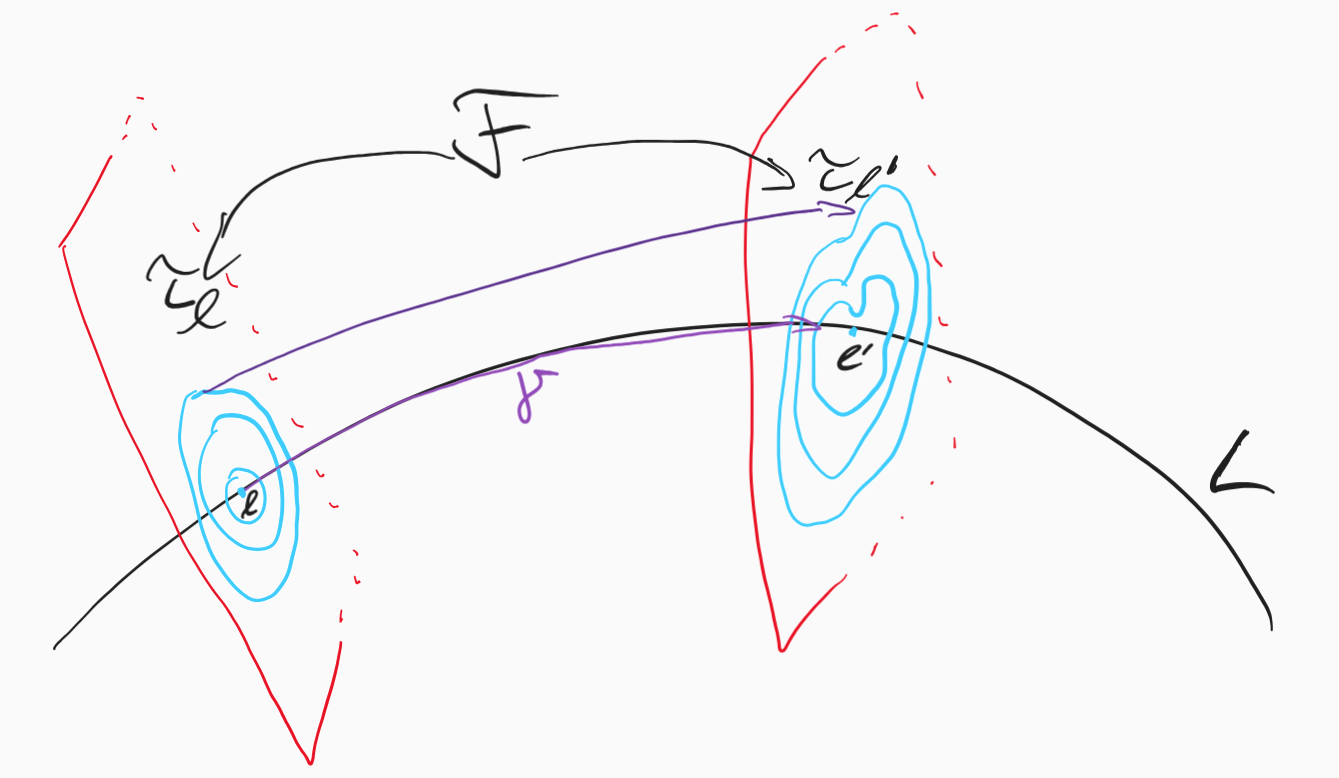
\includegraphics[width=.8\textwidth]{Foliation connection.png}
	%\caption{$\mathcal{F}$-connections}
	\label{fig:Foliation connection}
\end{figure}

\end{frame}

\setbeamertemplate{frame footer}{{Source of the existence of connection on normal bundle: Camille Laurent-Gengoux and Leonid Ryvkin, The holonomy of a singular leaf, \newline \textit{Selecta Mathematica 28}, no.\ 2, 45, 2022.}}

\begin{frame}{How to classify singular foliations?}
\begin{figure}[htbp]
	\centering
		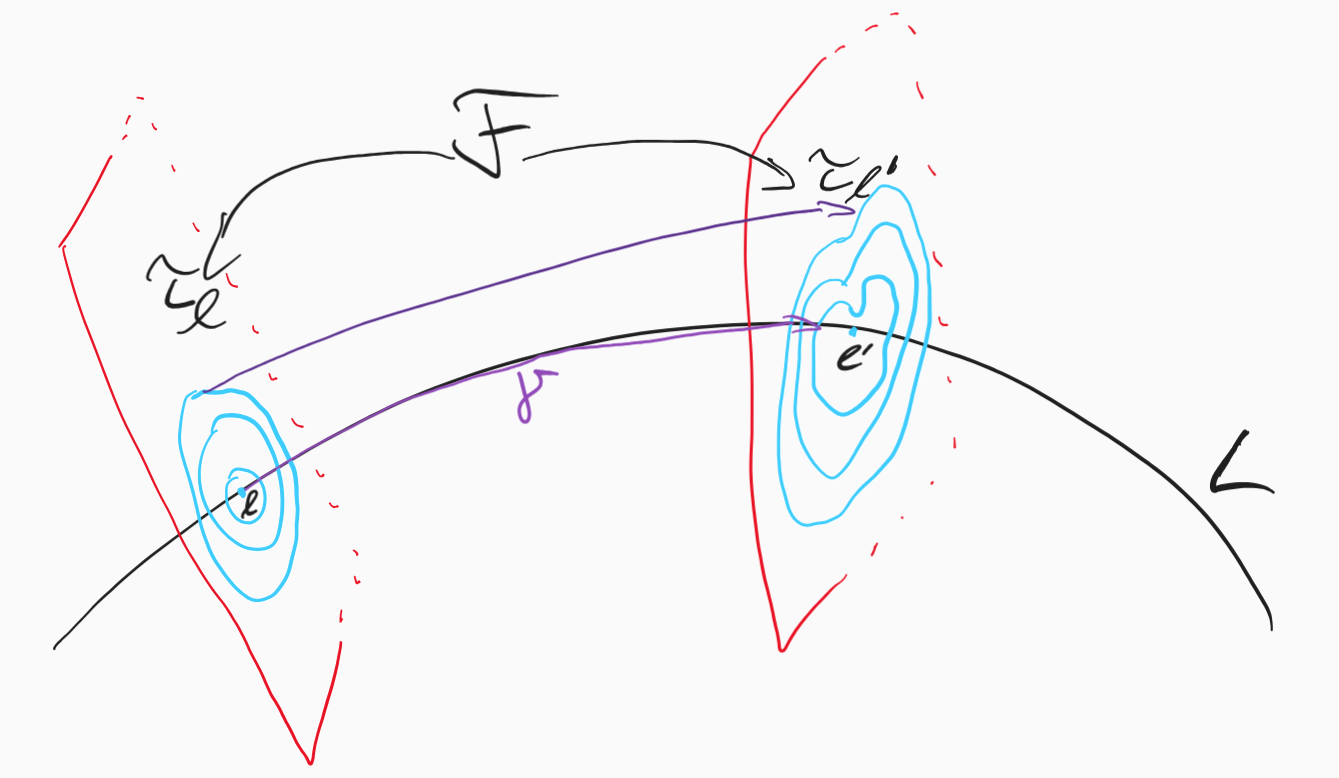
\includegraphics[width=0.4\textwidth]{Foliation connection.png}
	%\caption{$\mathcal{F}$-connections}
	\label{fig:Foliation connection Zwei}
\end{figure}

\begin{remark}[{[C.\ L.-G., S.-R.\ F.]}]
There is a connection on the normal bundle of a leaf $L$ preserving the foliation!
\begin{itemize}
	\item Transverse structure is unique: Classify singular foliation $\mathcal{F}$ like a bundle!
	\item Connection is a multiplicative Yang-Mills connection: Use curved gauge theory!
\end{itemize}
\end{remark}

\end{frame}

\subsection{Result}
\setbeamertemplate{frame footer}{}
{
%\setbeamertemplate{footline}{}
%\begin{frame}{Result}
%\begin{block}{Theorem ([C.\ L.-G., S.-R.\ F.])}
%\vspace{.5pt}
%Formal singular foliations with leaf $L$ and transverse model $(\mathbb{R}^d, \tau_l)$ are equivalent to:
%\begin{itemize}
	%\item A Galois cover $L'$ over $L$ with structural group $K$
	%\item A short exact sequence of groups
	%\begin{center}
		%\begin{tikzcd}[ampersand replacement=\&]
		%\mathup{Inner}(\tau_l) \arrow[hook]{r}
		%\&
		%H \arrow[two heads]{r}
		%\&
		%K
		%\end{tikzcd}
	%\end{center}
	%\item A principal $H$-bundle $P$ over $L$
%\end{itemize}
%\end{block}
%\end{frame}


%\begin{frame}
%\begin{remark}[Classification of curved Yang-Mills gauge theories]
%If $\mathcal{G}$ acts faithfully on the normal bundle $\mathcal{T}$, preserving $L$, then a curved Yang-Mills gauge theory can be flattened if and only if there is flat lift .
%\end{remark}
%
%\begin{table}[h!]
		%\begin{tabularx}{\textwidth}{X X}
			%\rowcolor{gray}
			%Curved YM Gauge Theory & Singular Foliations $\mathcal{F}$ \\
			%Multiplicative Yang-Mills connection & $\mathcal{F}$-connection \\
			%\rowcolor{Gray}
			%Flat gauge theory & Flat singular foliation \\
			%Field redefinition of connection on $\mathcal{G}$ & Different choice of $\mathcal{F}$-connection
		%\end{tabularx}
%\end{table}
%\end{frame}

}

\begin{frame}[standout]
\thispagestyle{empty}
\topmargin -3.46 cm
\vspace*{\fill}
\begin{center}
\huge \textbf{Thank you!}
\end{center}
\vspace*{\fill}
\end{frame}

\appendix

\begin{frame}[fragile]{Classification of singular foliations}
\begin{block}{Theorem ([C.\ L.-G., S.-R.\ F.])}
\vspace{.5pt}
Formal singular foliations with leaf $L$ and transverse model $(\mathbb{R}^d, \tau_l)$ are equivalent to:
\begin{itemize}
	\item A Galois cover $L'$ over $L$ with structural group $K$
	\item A short exact sequence of groups
	\begin{center}
		\begin{tikzcd}[ampersand replacement=\&]
		\mathup{Inner}(\tau_l) \arrow[hook]{r}
		\&
		H \arrow[two heads]{r}
		\&
		K
		\end{tikzcd}
	\end{center}
	\item A principal $H$-bundle $P$ over $L$
\end{itemize}
\end{block}

\end{frame}

\end{document}

